\begin{figure}[ht]
\centering
% Thesis-wide categorical color palette
% Usage: % Thesis-wide categorical color palette
% Usage: % Thesis-wide categorical color palette
% Usage: \input{figures/palette} in any figure file
%
% Muted primary colors -- print-friendly, visually distinct.
% Inspired by Cooper Union's red/blue primaries, softened for
% academic figures. Use palA-palC for data series in scatter
% plots, line charts, bar charts, etc.

\definecolor{palA}{HTML}{1F77B4}   % Tableau blue
\definecolor{palB}{HTML}{D62728}   % Tableau red
\definecolor{palC}{HTML}{2CA02C}   % Tableau green
 in any figure file
%
% Muted primary colors -- print-friendly, visually distinct.
% Inspired by Cooper Union's red/blue primaries, softened for
% academic figures. Use palA-palC for data series in scatter
% plots, line charts, bar charts, etc.

\definecolor{palA}{HTML}{1F77B4}   % Tableau blue
\definecolor{palB}{HTML}{D62728}   % Tableau red
\definecolor{palC}{HTML}{2CA02C}   % Tableau green
 in any figure file
%
% Muted primary colors -- print-friendly, visually distinct.
% Inspired by Cooper Union's red/blue primaries, softened for
% academic figures. Use palA-palC for data series in scatter
% plots, line charts, bar charts, etc.

\definecolor{palA}{HTML}{1F77B4}   % Tableau blue
\definecolor{palB}{HTML}{D62728}   % Tableau red
\definecolor{palC}{HTML}{2CA02C}   % Tableau green

\definecolor{nodeblue}{HTML}{B8D2E6}
\definecolor{nodeborder}{HTML}{5A87B5}
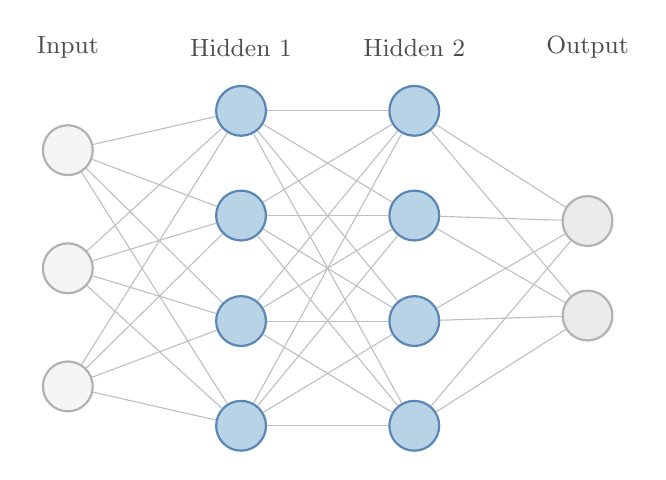
\begin{tikzpicture}[
    neuron/.style={circle, draw=nodeborder, thick, fill=nodeblue,
                   minimum size=18pt, inner sep=0pt},
    input/.style={circle, draw=black!30, thick, fill=black!4,
                  minimum size=18pt, inner sep=0pt},
    output/.style={circle, draw=black!30, thick, fill=black!8,
                   minimum size=18pt, inner sep=0pt},
    conn/.style={-, black!25},
    lbl/.style={font=\small, text=black!70},
    sublbl/.style={font=\scriptsize, text=black!50},
]

% === Main network ===

% Layer x-positions
\def\xin{0}
\def\xha{2.2}
\def\xhb{4.4}
\def\xout{6.6}

% --- Input layer (3 nodes) ---
\foreach \i/\ypos in {1/1.5, 2/0, 3/-1.5} {
    \node[input] (i\i) at (\xin, \ypos) {};
}
\node[lbl] at (\xin, 2.8) {Input};

% --- Hidden layer 1 (4 nodes) ---
\foreach \j/\ypos in {1/2.0, 2/0.67, 3/-0.67, 4/-2.0} {
    \node[neuron] (h1\j) at (\xha, \ypos) {};
}
\node[lbl] at (\xha, 2.8) {Hidden 1};

% --- Hidden layer 2 (4 nodes) ---
\foreach \k/\ypos in {1/2.0, 2/0.67, 3/-0.67, 4/-2.0} {
    \node[neuron] (h2\k) at (\xhb, \ypos) {};
}
\node[lbl] at (\xhb, 2.8) {Hidden 2};

% --- Output layer (2 nodes) ---
\foreach \l/\ypos in {1/0.6, 2/-0.6} {
    \node[output] (o\l) at (\xout, \ypos) {};
}
\node[lbl] at (\xout, 2.8) {Output};

% --- Connections ---
% Input -> Hidden 1
\foreach \i in {1,2,3} {
    \foreach \j in {1,2,3,4} {
        \draw[conn] (i\i) -- (h1\j);
    }
}
% Hidden 1 -> Hidden 2
\foreach \j in {1,2,3,4} {
    \foreach \k in {1,2,3,4} {
        \draw[conn] (h1\j) -- (h2\k);
    }
}
% Hidden 2 -> Output
\foreach \k in {1,2,3,4} {
    \foreach \l in {1,2} {
        \draw[conn] (h2\k) -- (o\l);
    }
}

\end{tikzpicture}
\vspace{6pt}
\caption{A fully connected network (multilayer perceptron) with three
  inputs, two hidden layers, and two outputs.}
\label{fig:mlp}
\end{figure}
